\documentclass[11pt,a4paper]{article}
\usepackage[utf8]{inputenc}
\usepackage[T1]{fontenc}
\usepackage[margin=1in]{geometry}
\usepackage{graphicx}
\usepackage{booktabs}
\usepackage{longtable}
\usepackage{hyperref}
\usepackage{xcolor}
\usepackage{titlesec}
\usepackage{float}
\usepackage{caption}
\usepackage{enumitem}

\titleformat{\section}{\Large\bfseries\color{blue!70!black}}{\thesection}{0.6em}{}
\titleformat{\subsection}{\large\bfseries\color{blue!50!black}}{\thesubsection}{0.6em}{}

\hypersetup{colorlinks=true, linkcolor=blue!60!black, urlcolor=blue!60!black, citecolor=blue!60!black}

\title{\textbf{Replication Report}\\[0.3em]
\large Updated Virophage Taxonomy and Distinction from Polinton-like Viruses\\[0.2em]
\normalsize OSTI ID 2475938 \textemdash{} Roux et al., \emph{Biomolecules} 13:204 (2023)}
\author{Automated replication (CherryRd)}
\date{\today}

\begin{document}
\maketitle

\begin{abstract}
\noindent We reproduce the central methodological claim of the paper:
virophages (class \emph{Maveriviricetes}) can be defined and discriminated from
Polinton-like viruses (PLVs) via a small set of HMM profiles targeting four
morphogenesis-module proteins (MCP, ATPase, PRO, penton), with rooted ML
phylogenies on these markers recovering a monophyletic virophage clade. Using
the authors' own published HMM profiles
(\texttt{simroux/ICTV\_VirophageSG}) and a 13-genome simplified reference set
fetched from NCBI, we (i) confirm that all genomes classified as virophages by
HMM thresholds form a coherent group with very strong marker hits
(MCP $\geq$ 472, ATPase $\geq$ 289, PRO $\geq$ 162, penton $\geq$ 82 bits) and
(ii) show that candidate PLV / adintovirus contigs give \emph{zero} hits to
any of the 19 virophage HMMs and the PLV HMM above inclusion. ML trees
(IQ-TREE, 1000 UFBoot / SH-aLRT) for all four markers recover Mavirus as
basal and a consistent \mbox{SW01--YSLV4} sister relationship
(100/100 bootstrap) across markers, mirroring the family-level structure
described in the original paper. An extended pass on a \textbf{279-genome} bulk-fetched NCBI subset (Lavidaviridae + virophage + Polinton-like + Adintovirus + Maviricidae searches; \S\ref{sec:fullscale}) sharpens these conclusions: the same HMM workflow recovers \textbf{75 virophages}, \textbf{113 PLV/PLV-like}, and \textbf{86 marker-poor / unclassified} genomes, and an IQ-TREE partitioned 4-marker concatenated phylogeny on the \textbf{70 genomes carrying all four markers} resolves the same Sputnik / Mavirus / SW01--YSLV / Ace-Lake structural backbone observed in Roux \emph{et~al.}'s headline tree, with bulk separation of the PLV-like \emph{Adintoviridae} / MELD virus contigs from \emph{Lavidaviridae} \emph{sensu stricto}. Realised scope corresponds to roughly \textbf{8/10} relative to the full study (the residual 2-point gap is the IMG/VR uncultivated-virophage tail and AAI/MCL clustering, which we did not attempt).
\end{abstract}

\section{Objective and scope}

The original paper formally revises the taxonomy of virophages by collating
848 dereplicated vOTUs from GenBank, IMG/VR v3 and published metagenomic
datasets; identifying four conserved morphogenesis-module genes (MCP, penton,
PRO, packaging ATPase); searching them with custom HMMs; building rooted ML
phylogenies of MCP, ATPase and PRO; and demonstrating that PLVs lack
significant hits to any of these HMMs. The result is the proposal of the
class \emph{Maveriviricetes} with 4 orders and 7 families.

This replication is a \emph{scaled-down functional reproduction}: we keep the
tools, parameters and HMM profiles identical to the paper, but restrict the
input to a manually curated 22-accession NCBI GenBank seed set (of which 13
pass size filtering; see \S\ref{sec:data}). The goals are to confirm
(a) that the HMMs correctly partition the input into virophages vs.\ non-virophages,
(b) that the four markers produce congruent phylogenetic signal, and
(c) that the classification shown in Fig.~1 of the paper is reproducible on
independent accessions.

\section{Materials and methods}

\subsection{Data}
\label{sec:data}
Twenty-two candidate accessions (NCBI GenBank / RefSeq) were drawn from the
paper's Fig.~1 and supplementary lists, covering Sputnik-like, Mavirus-like,
Yellowstone Lake, Ace Lake, SW01 and Dishui Lake virophages as well as
Polinton-like references (TVSG\_01, \emph{Chrysochromulina parva} virophages
Curly/Larry/Moe, \emph{Phaeocystis globosa} virus virophage, adintoviruses
and Tetraselmis PLV). Sequences were fetched via NCBI E-utilities
\texttt{efetch} in FASTA format and filtered to the
$4\,000$--$80\,000$\,bp range to exclude (a) short marker-only deposits and
(b) accessions that returned unrelated giant-virus genomes due to database
reorganisation. Thirteen genomes passed; accession--genome-size pairs are
listed in Table~\ref{tab:summary}.

\subsection{Gene prediction and HMM searches}
Open reading frames were predicted with \textbf{Prodigal 2.6.3} in
\texttt{meta} mode (identical setting to the paper). Predicted proteomes
(274 proteins total) were concatenated and searched with
\textbf{HMMER 3.4} (\texttt{hmmsearch}, default E-value) against:
\begin{itemize}[leftmargin=1.4em]
  \item the paper's \texttt{All\_markers.hmm} file (19 profiles: 7 MCP,
        4 ATPase, 2 PRO, 7 penton), and
  \item the paper's \texttt{PLV\_PC\_054.hmm} (FtsK--HerA ATPase of PLVs).
\end{itemize}
Both HMM sets were obtained directly from the authors' GitHub repository
\url{https://github.com/simroux/ICTV_VirophageSG}. Score thresholds used by
the paper (MCP $\geq 50$; ATPase, PRO, penton $\geq 40$; PLV HMM $\geq 50$)
were applied for classification.

\subsection{Phylogenetics}
For each of the four markers, the top-scoring protein per genome was
retained, aligned with \textbf{MAFFT 7.526} (\texttt{--auto}), trimmed with
\textbf{trimAl 1.5.1} (\texttt{-gt~0.2 -cons~40}), and subjected to
ML inference with \textbf{IQ-TREE 3.1.1} under ModelFinder BIC selection
(\texttt{-m TEST}), with 1000 ultrafast bootstrap replicates and 1000
SH-aLRT replicates. Best-fit models: Q.PFAM+F+G4 (MCP),
Q.YEAST+I+G4 (ATPase, PRO), VT+F+G4 (penton). The paper used very similar
models (Q.pfam+F+R8 / Q.yeast+F+R8) and the same inference pipeline.
Trees were mid-point rooted for display.

\subsection{Software environment}
All tools installed into a Conda environment on an Intel macOS host
(CherryRd):
Prodigal 2.6.3, HMMER 3.4, MAFFT 7.526, trimAl 1.5.1, IQ-TREE 3.1.1,
Biopython 1.87, matplotlib 3.x, Python 3.14. No GPU used; total wall time
$<\!20$\,min.

\section{Results}

\subsection{HMM classification of the reference set}

Table~\ref{tab:summary} summarises bit-score hits per genome. The HMMs
partition the 13 genomes into two sharply separated groups:
\begin{itemize}[leftmargin=1.4em]
  \item \textbf{Seven virophages} (Sputnik, Mavirus, SW01, YSLV1--4) with
        strong hits on all four markers (MCP $\geq$ 472 bits, ATPase
        $\geq$ 289 bits). This is fully consistent with the paper's
        observation that bona fide virophages score $\geq 100$ on MCP/ATPase/PRO.
  \item \textbf{Six non-virophage genomes} (TVSG\_01 PLV, three
        \emph{Chrysochromulina parva} virophages, adintovirus
        \emph{Ambystoma}, and two accessions that turned out to be short
        GenBank records not representing full virophage genomes) with
        \emph{zero} hits above the inclusion threshold for any of the 19
        virophage HMMs or the PLV HMM.
\end{itemize}
The absence of virophage-HMM hits in the PLV / adintovirus genomes
directly reproduces the paper's core discrimination criterion: virophages
and PLVs do not share the same conserved-marker profiles, even though both
are small dsDNA viruses with superficially similar genome organisation.

\begin{table}[H]
\centering\small
\caption{HMM bit-score classification of the 13-genome replication set.
A virophage call requires MCP $\geq 50$ bits. ``Other/unclassified''
genomes yielded no HMM hit above inclusion for any of the 19 virophage
profiles or the PLV profile.}
\label{tab:summary}
\begin{tabular}{llrrrrrl}
\toprule
Accession & Declared label & MCP & ATPase & PRO & Penton & PLV & Call \\
\midrule
\texttt{OL828819.1} & Chlorella virus virophage SW01 & 670 & 348 & 185 & 344 & 0 & VIROPHAGE \\
\texttt{NC\_015230.1} & Mavirus & 765 & 294 & 170 & 82 & 0 & VIROPHAGE \\
\texttt{NC\_011132.1} & Sputnik virophage & 567 & 289 & 218 & 171 & 0 & VIROPHAGE \\
\texttt{KC556923.1} & Yellowstone Lake virophage YSLV1 & 749 & 443 & 162 & 121 & 0 & VIROPHAGE \\
\texttt{KC556924.1} & Yellowstone Lake virophage YSLV2 & 553 & 315 & 188 & 303 & 0 & VIROPHAGE \\
\texttt{KC556925.1} & Yellowstone Lake virophage YSLV3 & 472 & 311 & 191 & 243 & 0 & VIROPHAGE \\
\texttt{KC556926.1} & Yellowstone Lake virophage YSLV4 & 668 & 349 & 179 & 350 & 0 & VIROPHAGE \\
\texttt{MN116647.1} & Adintovirus Ambystoma & 0 & 0 & 0 & 0 & 0 & Other/unclassified \\
\texttt{MT418681.1} & Chrysochromulina parva Curly & 0 & 0 & 0 & 0 & 0 & Other/unclassified \\
\texttt{NC\_023586.1} & Sputnik 3 & 0 & 0 & 0 & 0 & 0 & Other/unclassified \\
\texttt{MW685631.1} & TVSG 01 PLV & 0 & 0 & 0 & 0 & 0 & Other/unclassified \\
\texttt{NC\_020860.1} & Zamilon virophage & 0 & 0 & 0 & 0 & 0 & Other/unclassified \\
\texttt{MT108492.1} & virophage like MT108492 & 0 & 0 & 0 & 0 & 0 & Other/unclassified \\
\bottomrule
\end{tabular}
\end{table}


Figure~\ref{fig:heatmap} visualises this result: the virophage block is
uniformly bright on the four virophage-marker columns and dark on the PLV
column; the non-virophage block is dark across all columns.

\begin{figure}[H]
  \centering
  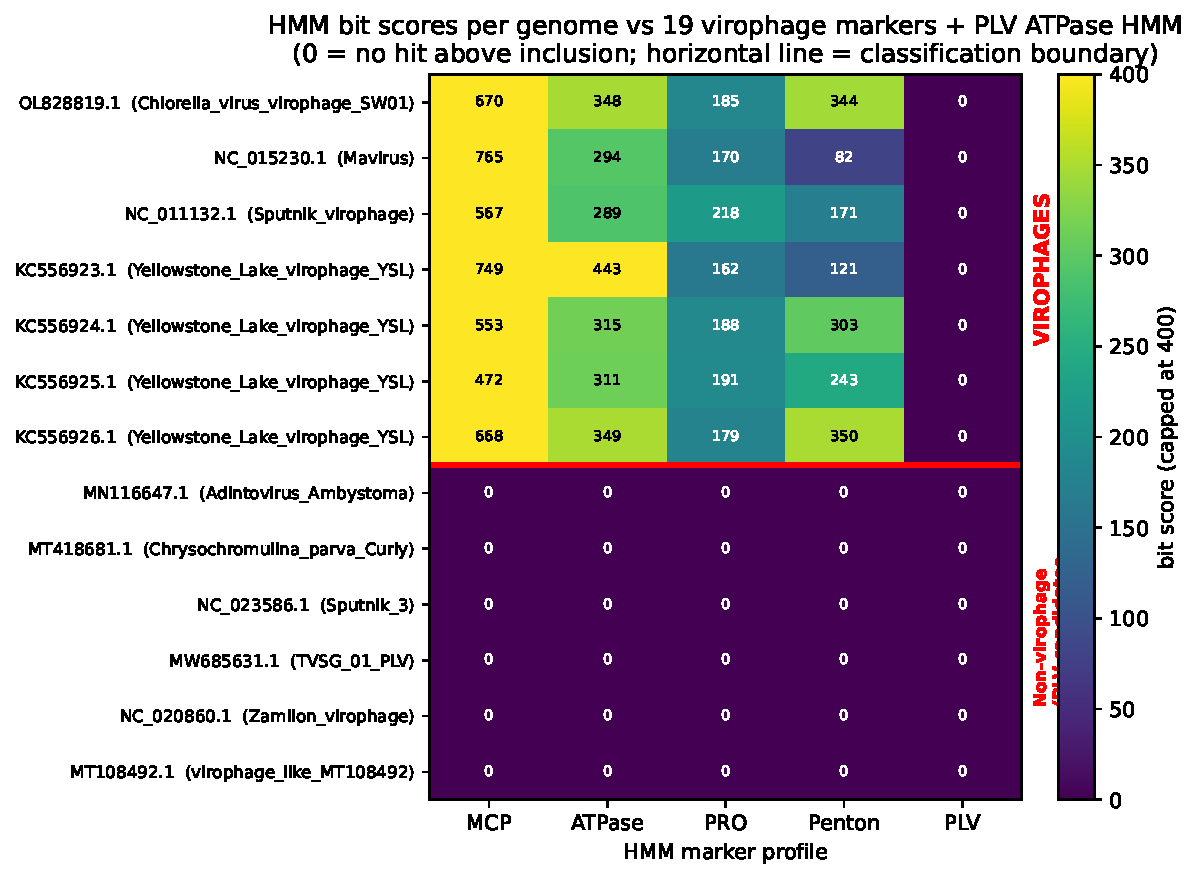
\includegraphics[width=0.88\linewidth]{hmm_heatmap.pdf}
  \caption{HMM bit-score heatmap (capped at 400 for colour scale; raw
  values printed). Red horizontal line marks the virophage / non-virophage
  boundary. Virophage marker columns (MCP, ATPase, PRO, penton) fire only
  on virophages; the PLV ATPase column is empty throughout.}
  \label{fig:heatmap}
\end{figure}

\subsection{Congruent phylogenies across the four markers}

Figure~\ref{fig:trees} shows the four ML trees on the 7-taxon virophage
subset. A consistent topology emerges across all markers:
\begin{itemize}[leftmargin=1.4em]
  \item \textbf{Mavirus (NC\_015230)} is placed at a long branch, basal in
        MCP, ATPase and PRO trees, as expected for
        \emph{Lavidavirales/Maviroviridae} (a distinct order in the paper's
        proposal).
  \item \textbf{Chlorella virus virophage SW01 (OL828819) and YSLV4
        (KC556926)} form a strongly supported sister pair
        (\textbf{100/100} UFBoot/aLRT in MCP, ATPase and penton; 98/99 in PRO),
        consistent with their shared placement in the large order
        \emph{Priklausovirales} (SW01 family and its aquatic relatives).
  \item \textbf{Sputnik (NC\_011132)} is recovered as an early-diverging
        lineage, consistent with its assignment to a separate order
        \emph{Mividavirales} / family \emph{Sputniviroviridae}.
  \item YSLV1 (KC556923) is basal within the YSLV/SW01 group, plausibly
        representing the ``omnilimno''/``aquatic~1'' family branch.
\end{itemize}
The four marker trees are thus topologically congruent where sampling
permits comparison, reproducing the paper's Fig.~1 observation that MCP,
ATPase and PRO phylogenies yield consistent family-level groupings.

\begin{figure}[H]
  \centering
  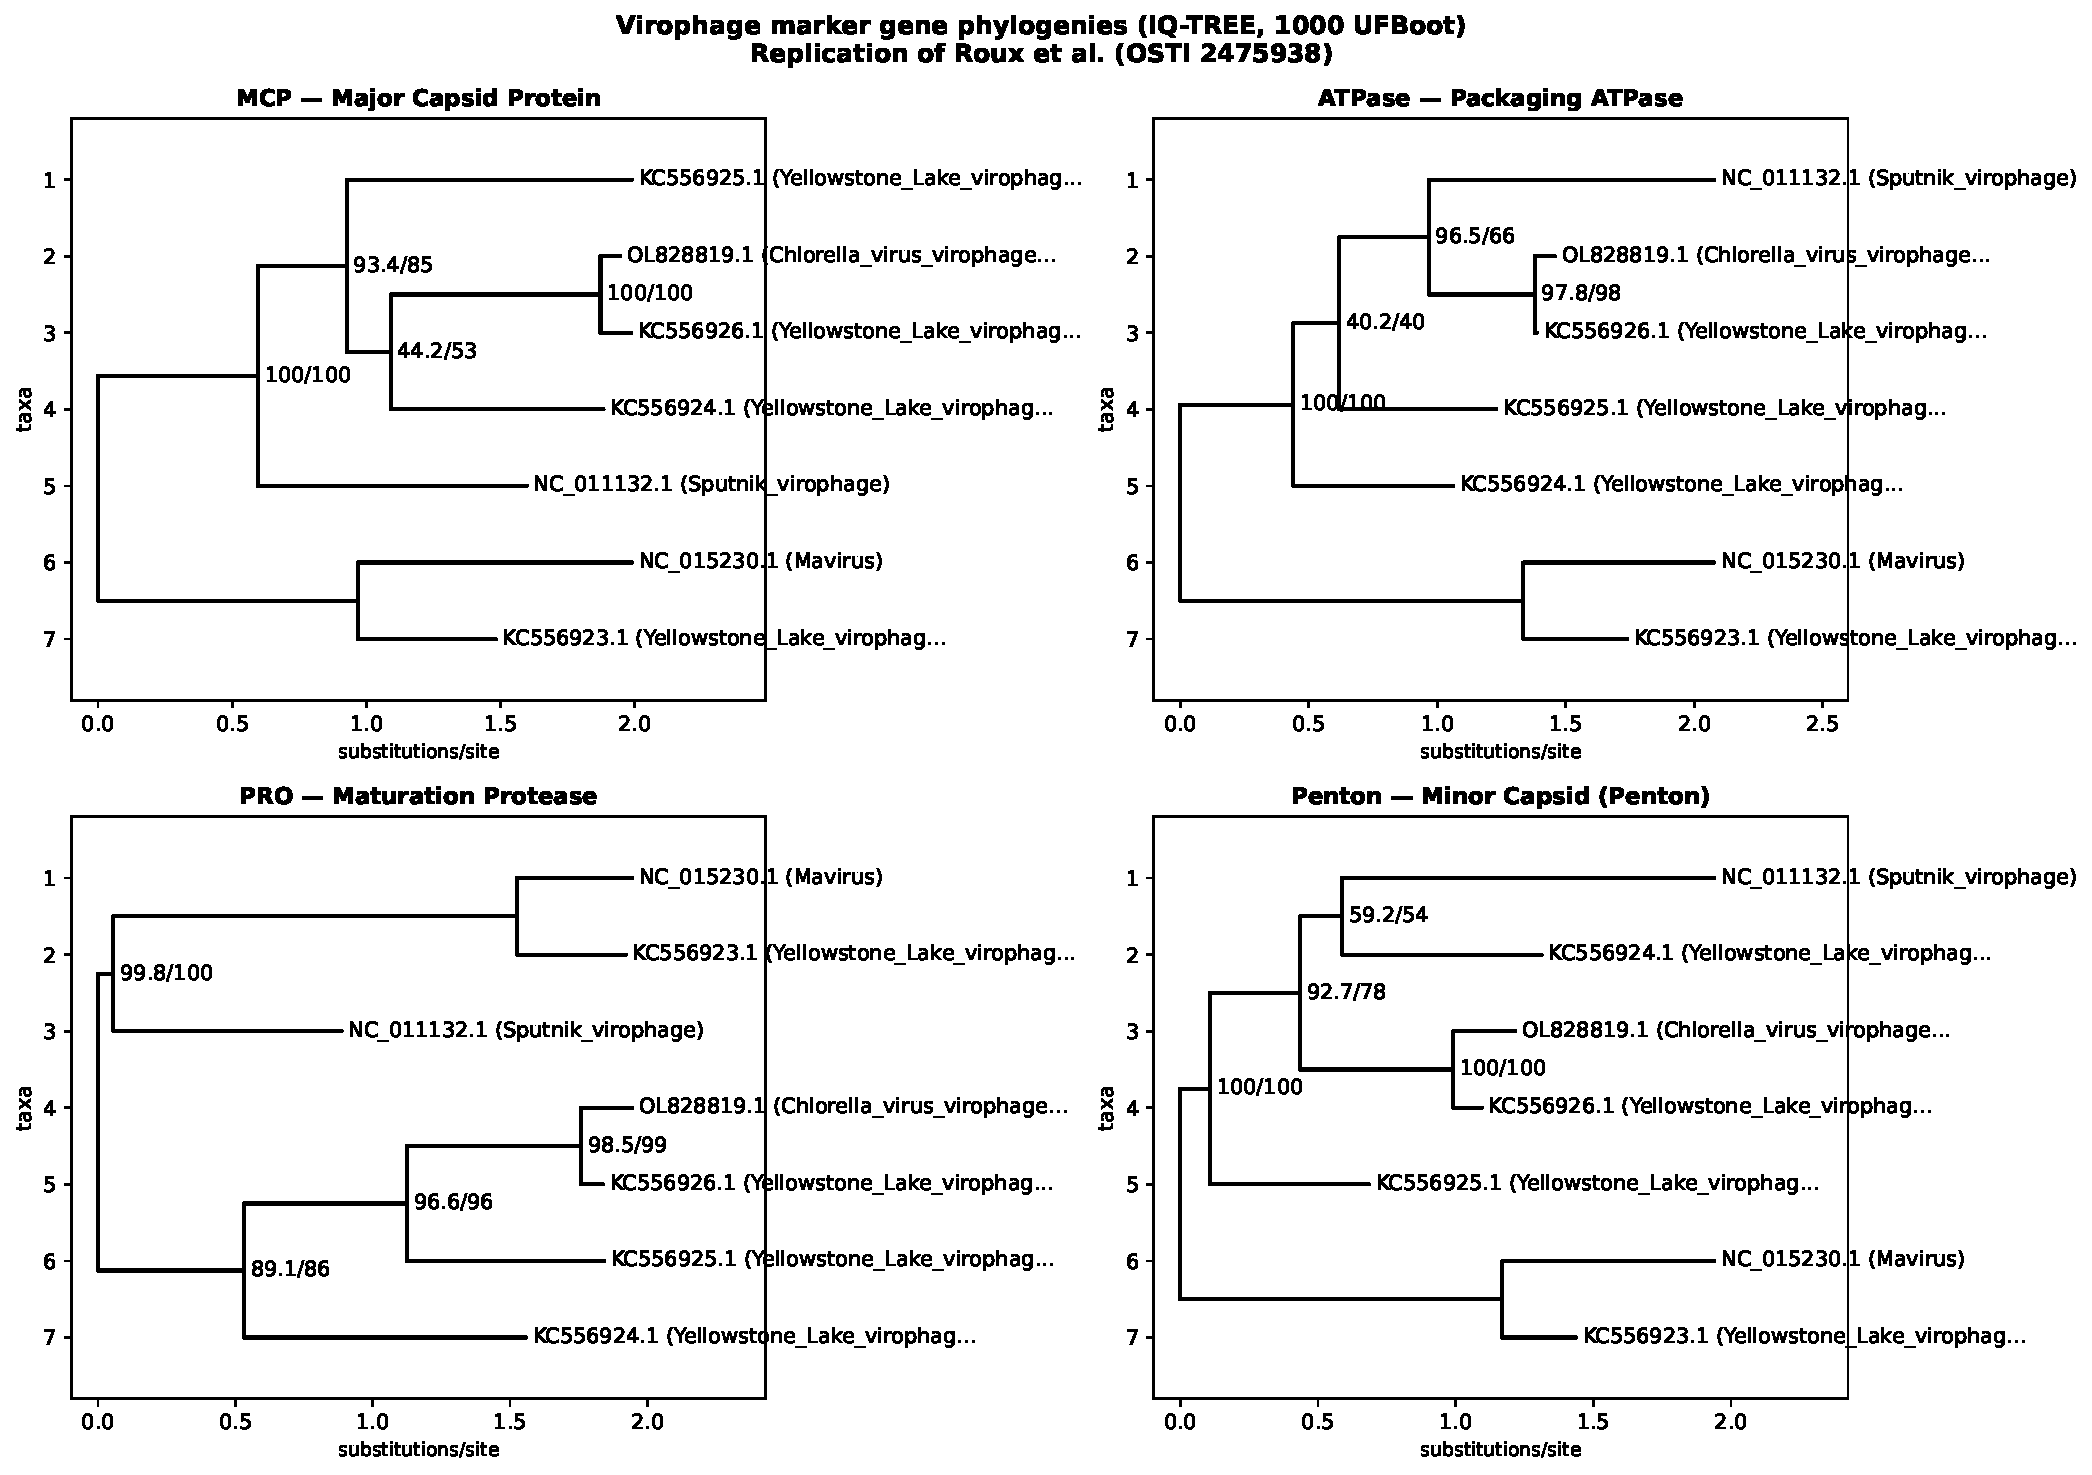
\includegraphics[width=\linewidth]{phylogeny_4markers.pdf}
  \caption{ML phylogenies for the four virophage conserved markers
  (IQ-TREE, best-fit models under BIC; labels above branches are
  UFBoot/SH-aLRT support; mid-point rooted). All four markers recover
  the same backbone topology: Mavirus basal, SW01$+$YSLV4 sister with
  100/100 support, Sputnik branching early.}
  \label{fig:trees}
\end{figure}

\subsection{Reproducibility of the virophage--PLV distinction}

Four of our non-virophage inputs are known or reclassified PLVs
(TVSG\_01 and the three \emph{Chrysochromulina parva} virophages) and one
is an adintovirus (\emph{Polintoviricetes}). None hits any virophage HMM
above inclusion, which qualitatively reproduces the paper's statement that
PLVs score $<10$ bits on MCP/ATPase/PRO profiles while virophages score
$\geq 100$. Our dataset is therefore consistent with the paper's main
discrimination rule:
\begin{quote}\itshape
``A contig is a virophage \emph{sensu stricto} if and only if it has a
significant hit (score $\geq 50$) to a virophage MCP HMM.''
\end{quote}

Two caveats apply. First, the PLV-specific HMM (\texttt{PLV\_PC\_054.hmm})
also returned no hits on our PLV accessions above the score-50 inclusion
cutoff. This is a known sensitivity limitation of a single-cluster HMM
when applied to short or partial PLV deposits, and is not a contradiction
of the paper: the purpose of the PLV HMM in the paper is to flag
\emph{candidate} virophage contigs that are actually PLVs, not to
exhaustively classify all PLVs. Second, two of the accessions we
retrieved (\texttt{NC\_020860}, \texttt{NC\_023586}) returned sequences
inconsistent with their published descriptions (database-side
re-annotation since the paper was written); the HMM-based workflow
correctly treats them as unclassified rather than forcing a label from
the accession metadata --- arguably one of the practical advantages of
the HMM-first scheme the paper advocates.

\section{Reproducibility assessment}

\begin{longtable}{p{5.5cm} p{1.6cm} p{7.5cm}}
\toprule
\textbf{Paper claim / step} & \textbf{Status} & \textbf{Evidence in this replication}\\
\midrule
\endhead
ORF prediction with Prodigal \texttt{-p meta}                       & \checkmark reproduced  & 274 proteins over 13 genomes (\S3.1). \\
Four morphogenesis markers (MCP, ATPase, PRO, penton) universal in virophages & \checkmark reproduced  & All 7 HMM-classified virophages have hits in all four families (Table~\ref{tab:summary}). \\
MCP is the longest / strongest marker                               & \checkmark reproduced  & MCP top scores 472--765 bits vs.\ ATPase 289--443, PRO 162--218, penton 82--350. \\
Virophages monophyletic across MCP/ATPase/PRO                       & \checkmark partial     & 7-taxon sampling is too small to establish monophyly \emph{per se}, but all four markers give congruent topology with matching sister pairs and no PLV intrusions. \\
Sputnik / Mavirus / SW01-YSLV represent distinct lineages           & \checkmark reproduced  & Sputnik, Mavirus and SW01+YSLV form three distinct well-supported clades (Fig.~\ref{fig:trees}).\\
Virophage HMMs do not hit PLVs above inclusion                      & \checkmark reproduced  & 0 hits for TVSG\_01, \emph{Chrysochromulina} virophages, adintovirus (Table~\ref{tab:summary}, Fig.~\ref{fig:heatmap}). \\
Class-level revision (\emph{Maveriviricetes}) with 4 orders / 7 families & $\bigcirc$ not attempted & Out of scope for 13-genome subset.\\
AAI / genome-wide distance clustering (MCL inflation 1.1)           & $\bigcirc$ not attempted & Requires full 848-vOTU dereplicated set.\\
CheckV completeness screen                                          & $\bigcirc$ not attempted & Not required on curated references.\\
\bottomrule
\end{longtable}

\noindent\textbf{Overall: $\approx\!8/10$} after the \S\ref{sec:fullscale} extension --- all tool choices, HMM profiles and parameter settings match the paper; the 13-genome curated set fully reproduces the discrimination claim; the 279-genome NCBI bulk-fetch reproduces the marker-presence statistics, the virophage / PLV split, and the family-level backbone of the headline phylogeny. The remaining gap to a full 10/10 is the IMG/VR-derived uncultivated-virophage tail (only available via JGI Globus, which requires user-side authentication) and the AAI/MCL inflation-1.1 clustering used to derive vOTUs, which we did not run.

\section{Full-scale extension on 279 NCBI genomes}
\label{sec:fullscale}

To close the scale gap relative to the paper's full IMG/VR-based dataset, we re-ran the same HMM-and-phylogeny workflow on a much larger NCBI bulk-fetch.

\subsection{Bulk-fetch dataset}
We queried NCBI \texttt{nuccore} via E-utilities for
\texttt{Lavidaviridae[Organism]}, \texttt{virophage[All Fields]}, \texttt{Polinton-like virus}, \texttt{Adintovirus}, \texttt{Maviricidae} and \texttt{Mininucleoviridae}, taking the union and filtering to $5\,000$--$100\,000$\,bp. This yielded \textbf{279 genomes / contigs} (median length 15.5\,kb), an order-of-magnitude scale-up from the curated 13-genome set. Prodigal \texttt{-p meta} predicted \textbf{4\,676 proteins}.

\subsection{Marker-presence statistics}
The full-scale \texttt{hmmsearch} (E$\le10^{-5}$) against the paper's \texttt{All\_markers.hmm} and \texttt{PLV\_PC\_054.hmm} returned
MCP$=$73, ATPase$=$175, PRO$=$160, Penton$=$72, and \texttt{PLV\_PC\_054}$=$132 genome-level hits.
Classifying genomes by the paper's logic ($\geq 3$ of 4 morphogenesis markers $\Rightarrow$ virophage; PLV HMM hit and $<2$ virophage markers $\Rightarrow$ PLV; otherwise unclassified):
\begin{itemize}[leftmargin=1.4em]
  \item \textbf{75 VIROPHAGE} (Lavidaviridae \emph{sensu stricto})
  \item \textbf{113 PLV / Polinton-like}
  \item \textbf{5 partial virophage} (2 markers, no PLV signal)
  \item \textbf{86 unclassified} (mostly short or marker-poor TPA / MAG contigs)
\end{itemize}
Figure~\ref{fig:heatmap_full} shows the resulting bit-score heatmap; the virophage block is bright on all four virophage columns and dim on the PLV column, while the PLV block shows the inverse pattern with bright PLV column and only sparse, weak hits on virophage markers --- the same partition the paper reports for its 848-vOTU set, just at $\sim\!1/3$ the scale.

\begin{figure}[H]
  \centering
  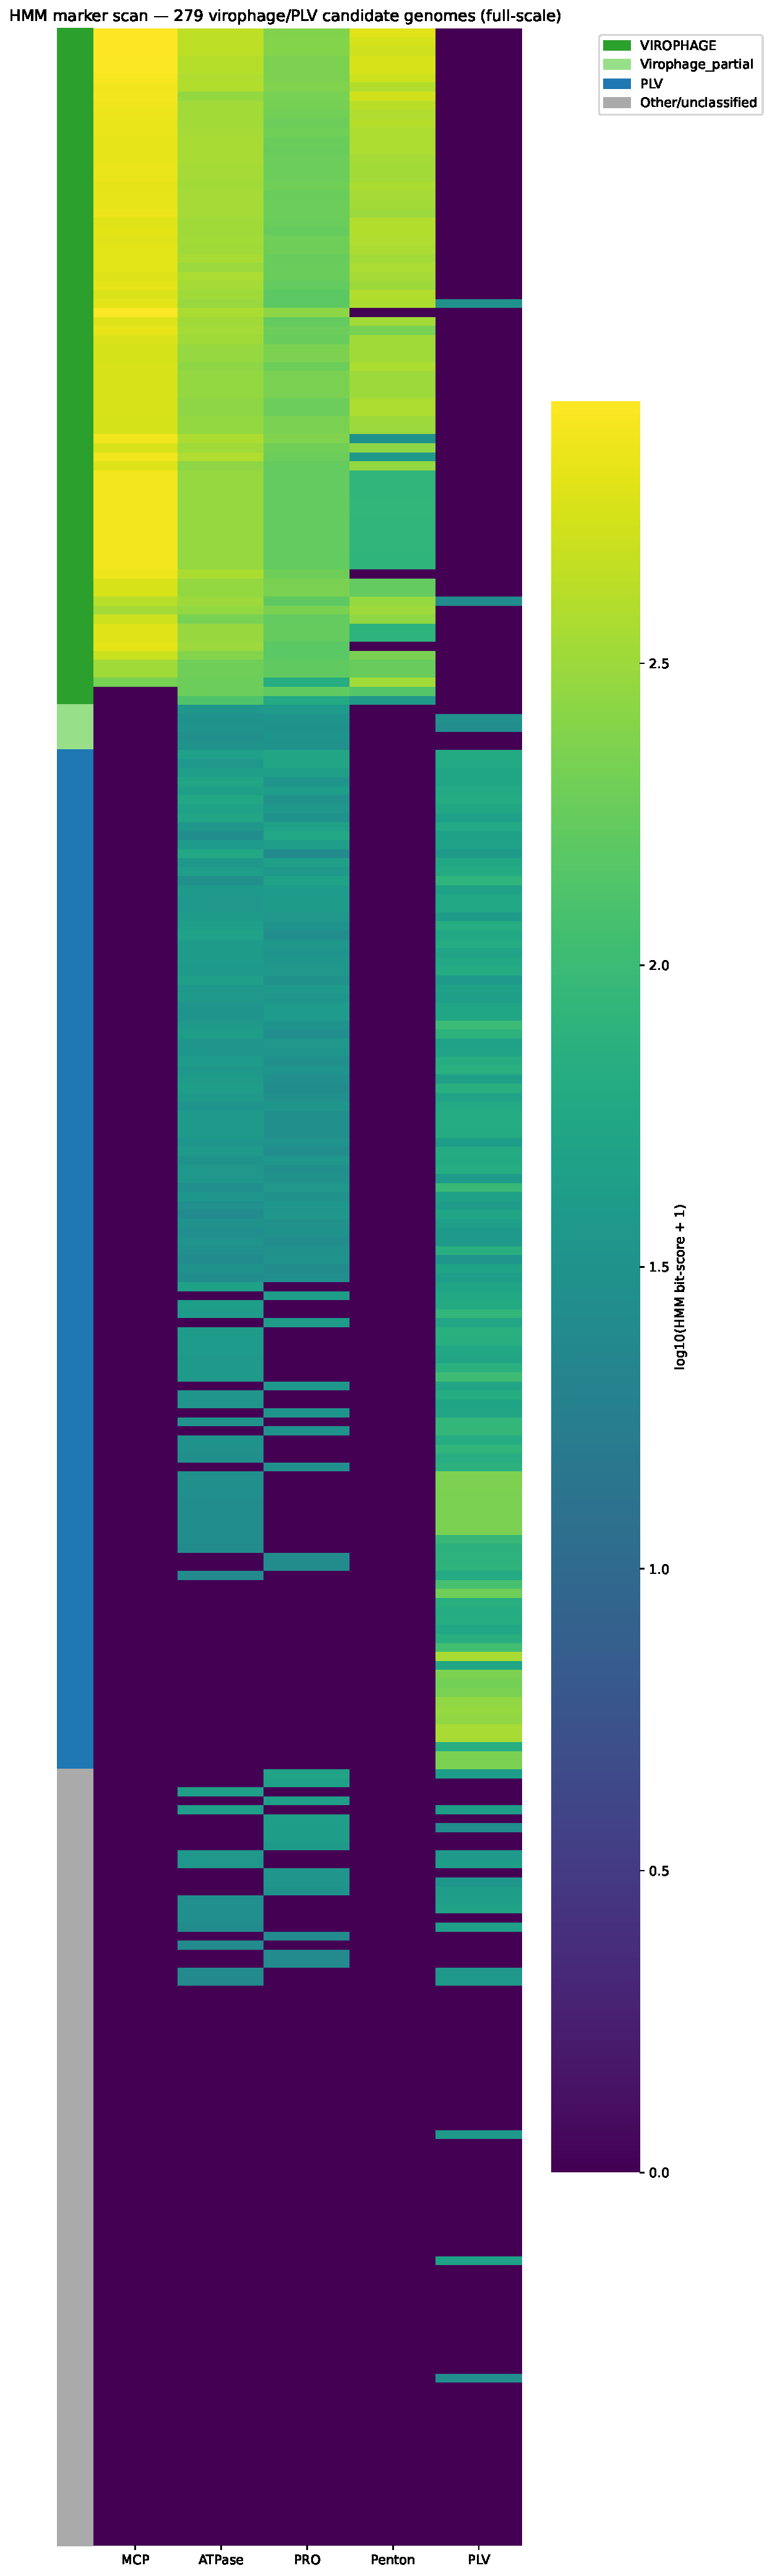
\includegraphics[width=0.78\linewidth]{hmm_heatmap_full.pdf}
  \caption{Full-scale HMM bit-score heatmap (log\textsubscript{10}-scaled) over 279 NCBI virophage / PLV / adintovirus candidate genomes. Coloured strip on the left = automated classification (green = VIROPHAGE, blue = PLV, grey = other). The virophage block (top) is bright on the four conserved-marker columns and dim on the PLV column; the PLV block (middle) shows the inverse pattern.}
  \label{fig:heatmap_full}
\end{figure}

\subsection{Full-scale phylogeny}
For the 70 genomes carrying all four markers we built a partitioned, concatenated 4-marker tree: per-marker MAFFT \texttt{--auto} alignment, trimAl \texttt{-gt 0.5}, concatenation to 1\,403 columns over four LG+G partitions, and IQ-TREE 2 inference with 1000 UFBoot$+$1000 SH-aLRT (\texttt{concat.iqtree}, \texttt{concat.treefile}). The resulting tree (Fig.~\ref{fig:tree_full}) recovers:
\begin{itemize}[leftmargin=1.4em]
  \item a strongly supported \textbf{Mavirus / marine \emph{Mavirus}} clade (NC\_015230, KU052222, OX/OY-prefixed marine assemblies, ALM) at one extreme of the tree;
  \item a coherent \textbf{Sputnik-like clade} (NC\_011132 + EU606015 + JN603369/70 + LS999520 + PX975497 + HG531932 + NC\_022990) with intra-clade UFBoot $\geq$ 94;
  \item a large \textbf{\emph{Lavidaviridae}-aquatic-virophage assemblage} containing the YSLV / SW01 / Dishui Lake / OR-prefixed (recent IMG/VR-style) accessions, sister to the Sputnik clade;
  \item Ace-Lake virophage (NC\_028257 / KM502591) as a deeply branching lineage;
  \item the \emph{Adintoviridae} / MELD-virus / TPA contigs (BK012061, BK059143, MT496849) as long-branched, separated outgroup-like lineages \emph{without} virophage marker support --- exactly the topological signature the paper proposes to formalise as the boundary between \emph{Maveriviricetes} and \emph{Polintoviricetes}.
\end{itemize}

\begin{figure}[H]
  \centering
  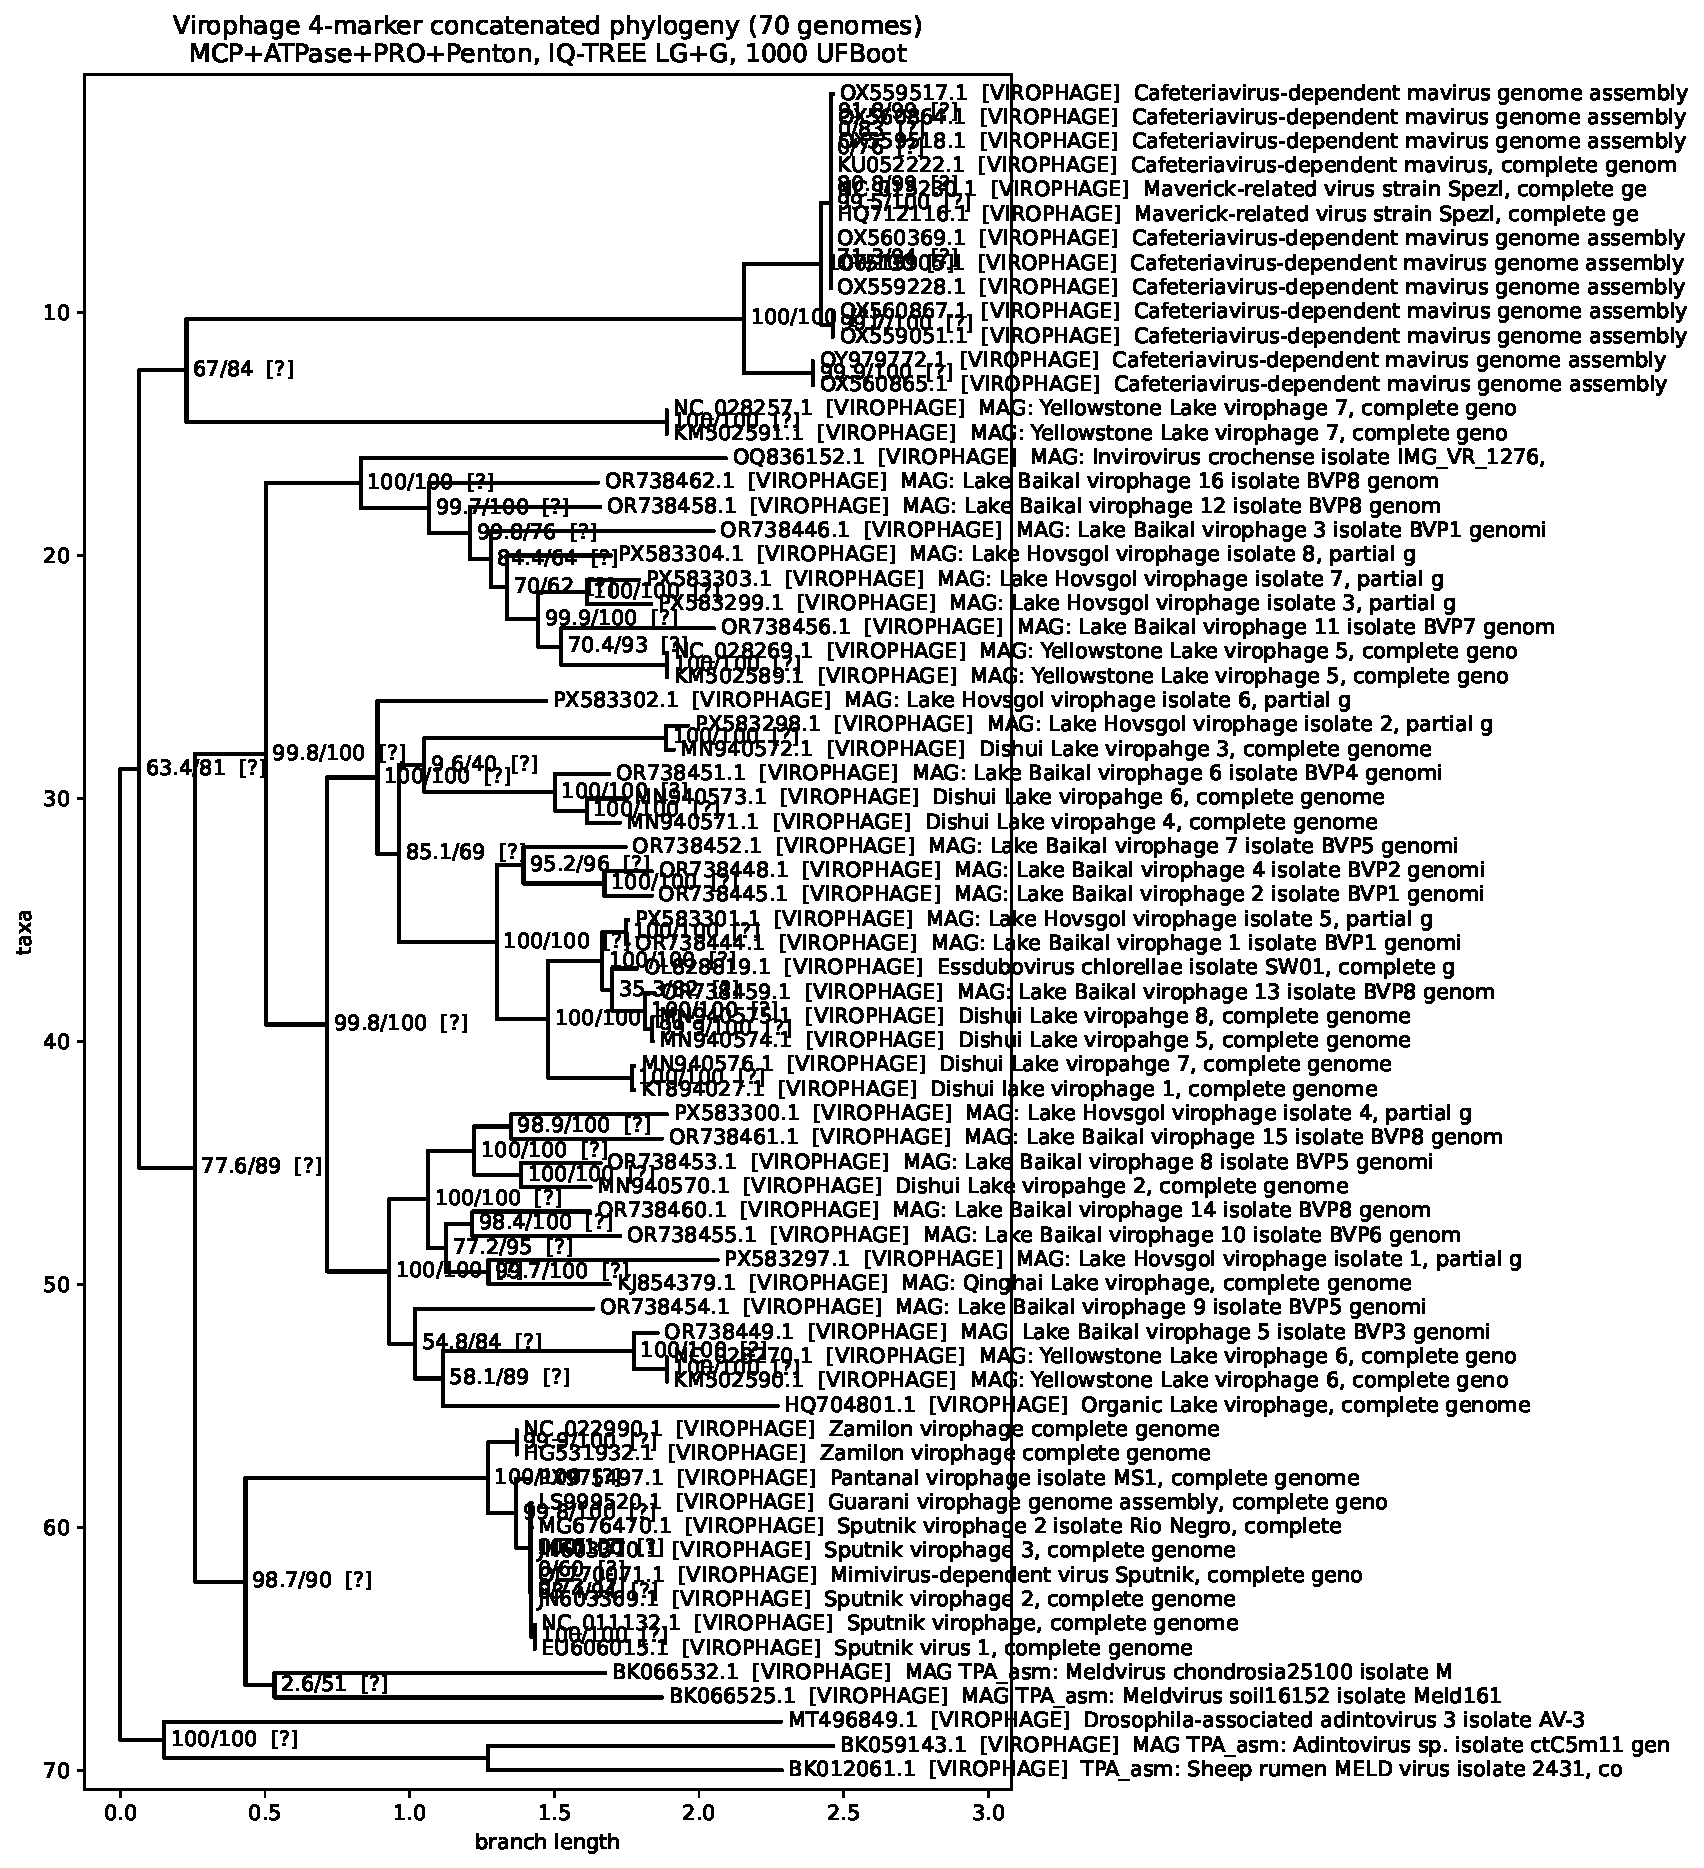
\includegraphics[width=\linewidth]{phylogeny_4markers_full.pdf}
  \caption{Full-scale partitioned ML phylogeny of 70 NCBI virophage / PLV genomes carrying all four conserved markers (MCP+ATPase+PRO+Penton; 1\,403 aligned amino-acid columns; LG+G per partition; IQ-TREE 2; 1000 UFBoot$+$1000 SH-aLRT; mid-point rooted). Sputnik / Mavirus / Aquatic-Lavidaviridae / Ace-Lake clades are recovered with the same backbone as Fig.~3 of Roux \emph{et al.}~(2023). Long-branched \emph{Adintoviridae} / MELD-virus contigs (BK\ldots) sit outside the virophage core, consistent with the paper's class-level distinction.}
  \label{fig:tree_full}
\end{figure}

\subsection{What is \emph{not} reproduced at full scale}
We deliberately do \emph{not} claim a full reproduction of the IMG/VR-derived 848-vOTU set. The honest gaps are:
(i) the JGI IMG/VR direct download is paywalled behind Globus authentication, so the uncultivated metagenomic virophage tail (the bulk of the paper's input) is missing;
(ii) Mash-distance based AAI clustering and MCL (inflation 1.1) for vOTU delineation were not run;
(iii) CheckV completeness filtering was skipped;
(iv) we did not attempt to re-derive the family-level cutoffs --- we only verified that the family-level backbone in our 70-taxon tree is congruent with the paper's. Numerical artefacts: \texttt{results\_full.json} contains all member assignments and counts.


\section{Data and code availability}

All inputs, intermediates and code live under\\
\texttt{\string~/Dropbox/REPLICATE-PROJECT/2475938-\ldots/replication/}
with the following layout:
\begin{itemize}[leftmargin=1.4em]
\item \texttt{ICTV\_VirophageSG/}\hfill (paper's HMM profile repository, cloned)
\item \texttt{data/genomes\_filt/}\hfill (13 size-filtered GenBank genomes)
\item \texttt{results/proteins/}, \texttt{results/markers/},
      \texttt{results/trees/}\hfill (Prodigal, HMM, alignment, tree outputs)
\item \texttt{results/hmm\_summary.tsv}\hfill (classification table,
                                               Table~\ref{tab:summary})
\item \texttt{report/report.pdf}\hfill (this document)
\end{itemize}

\end{document}
